پروژه یک برنامه‌ی \lr{React 18} با \lr{TypeScript} و \lr{Vite} است (داشبورد وضعیت سرویس‌ها) و طبق صورت سؤال {هیچ خطی از کد برنامه تغییر نکرده}؛ تنها فایل‌های مرتبط با داکر اضافه یا اصلاح شده‌اند.

\begin{figure}[H]
\centering
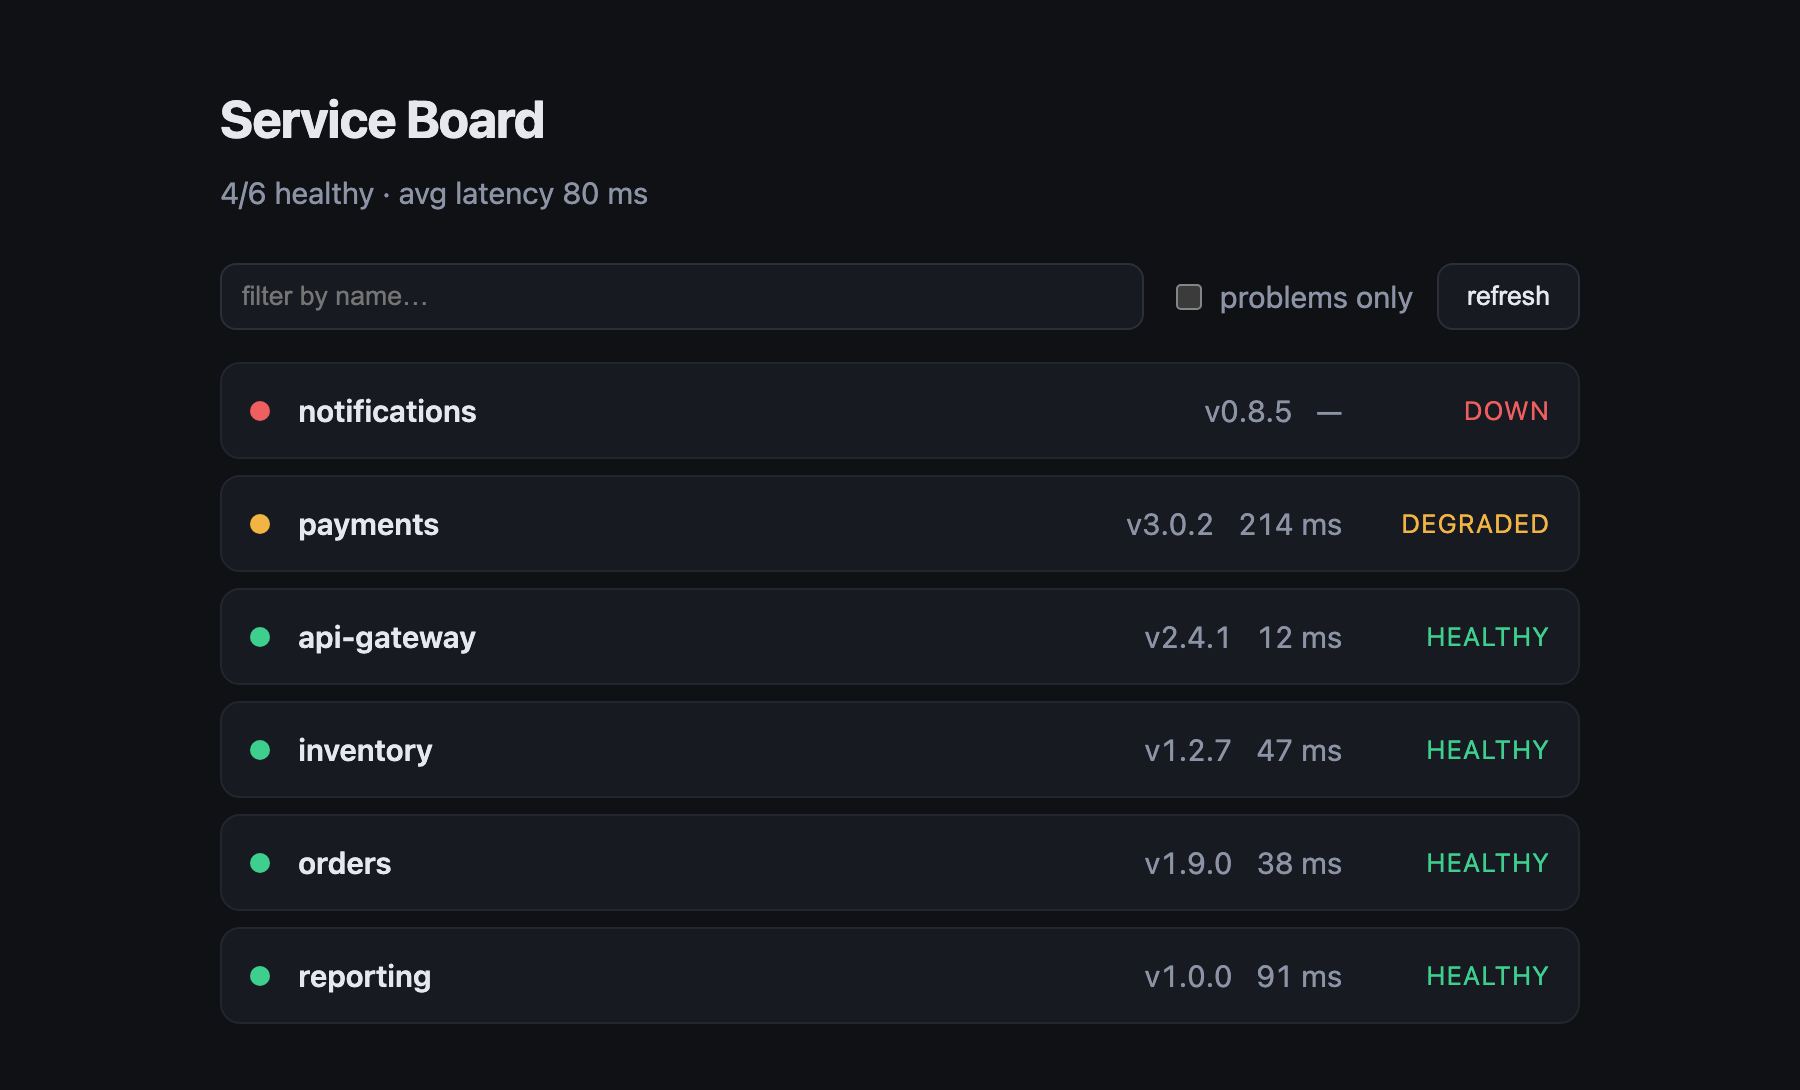
\includegraphics[width=0.62\textwidth]{figs/q5-app.png}
\caption{برنامه‌ای که داکرایز شده است، در حال سرو شدن از ایمیج بهینه‌شده روی \lr{nginx}.}
\end{figure}

\subsubsection*{مشکلات \lr{Dockerfile} اولیه}

\begin{lstlisting}[language=Docker]
FROM node:latest
WORKDIR /app
COPY . .
RUN npm install
RUN npm run build
CMD ["npm", "start"]
\end{lstlisting}

\begin{itemize}
	\item \lr{node:latest} هم غیرقابل تکرار است (فردا نسخه‌ی دیگری است) و هم حدود \lr{1.1GB} فقط پایه است.
	\item ایمیج نهایی شامل \lr{Node}، \lr{npm}، کل \lr{node\_modules} و سورس‌هاست، در حالی که خروجی واقعی فقط چند فایل ایستا در \lr{dist/} است.
	\item \lr{COPY . .} قبل از \lr{npm install} است؛ پس با تغییر یک کاراکتر در یک کامپوننت، لایه‌ی نصب وابستگی‌ها باطل و \lr{npm install} از نو اجرا می‌شود.
	\item نبود \lr{.dockerignore} یعنی \lr{node\_modules} میزبان هم وارد \lr{context} می‌شود؛ روی \lr{macOS/arm64} این فایل‌های باینری برای ایمیج \lr{linux} نامعتبرند.
	\item \lr{npm install} به‌جای \lr{npm ci}؛ ممکن است نسخه‌ها با \lr{lockfile} یکی نباشند.
	\item برنامه با کاربر \lr{root} و از طریق سرور توسعه‌ای \lr{vite preview} سرو می‌شود، نه یک وب‌سرور واقعی.
\end{itemize}

\subsubsection*{نسخه‌ی بهینه‌شده}

\begin{lstlisting}[language=Docker]
ARG NODE_VERSION=22.12.0
ARG NGINX_VERSION=1.27

FROM node:${NODE_VERSION}-alpine AS deps
WORKDIR /app
COPY package*.json ./
RUN --mount=type=cache,target=/root/.npm \
    npm ci --no-audit --no-fund

FROM node:${NODE_VERSION}-alpine AS build
WORKDIR /app
COPY --from=deps /app/node_modules ./node_modules
COPY . .
RUN npm run build

FROM nginx:${NGINX_VERSION}-alpine AS runtime
COPY nginx.conf /etc/nginx/conf.d/default.conf
COPY --from=build /app/dist /usr/share/nginx/html
EXPOSE 80
HEALTHCHECK --interval=30s --timeout=3s --start-period=5s --retries=3 \
    CMD wget --spider -q http://127.0.0.1/ || exit 1
CMD ["nginx", "-g", "daemon off;"]
\end{lstlisting}

\subsubsection*{مقایسه‌ی حجم و سرعت}

\begin{center}
\begin{tabular}{|l|r|r|r|}
\hline
 & {حجم ایمیج} & {بیلد کامل} & {بیلد پس از یک خط تغییر} \\
\hline
\lr{Dockerfile} اولیه & \lr{1.34 GB} (۱۲۷۴ مگابایت) & \lr{201 s} & \lr{12.7 s} \\
\hline
\lr{Dockerfile} بهینه & \lr{49.9 MB} (۴۷٫۵ مگابایت) & \lr{137 s} & \lr{1.9 s} \\
\hline
{بهبود} & {$\approx$ ۲۷ برابر کوچک‌تر} & $\approx$ ۱٫۵ برابر & {$\approx$ ۶٫۷ برابر سریع‌تر} \\
\hline
\end{tabular}
\end{center}

\begin{figure}[H]
\centering
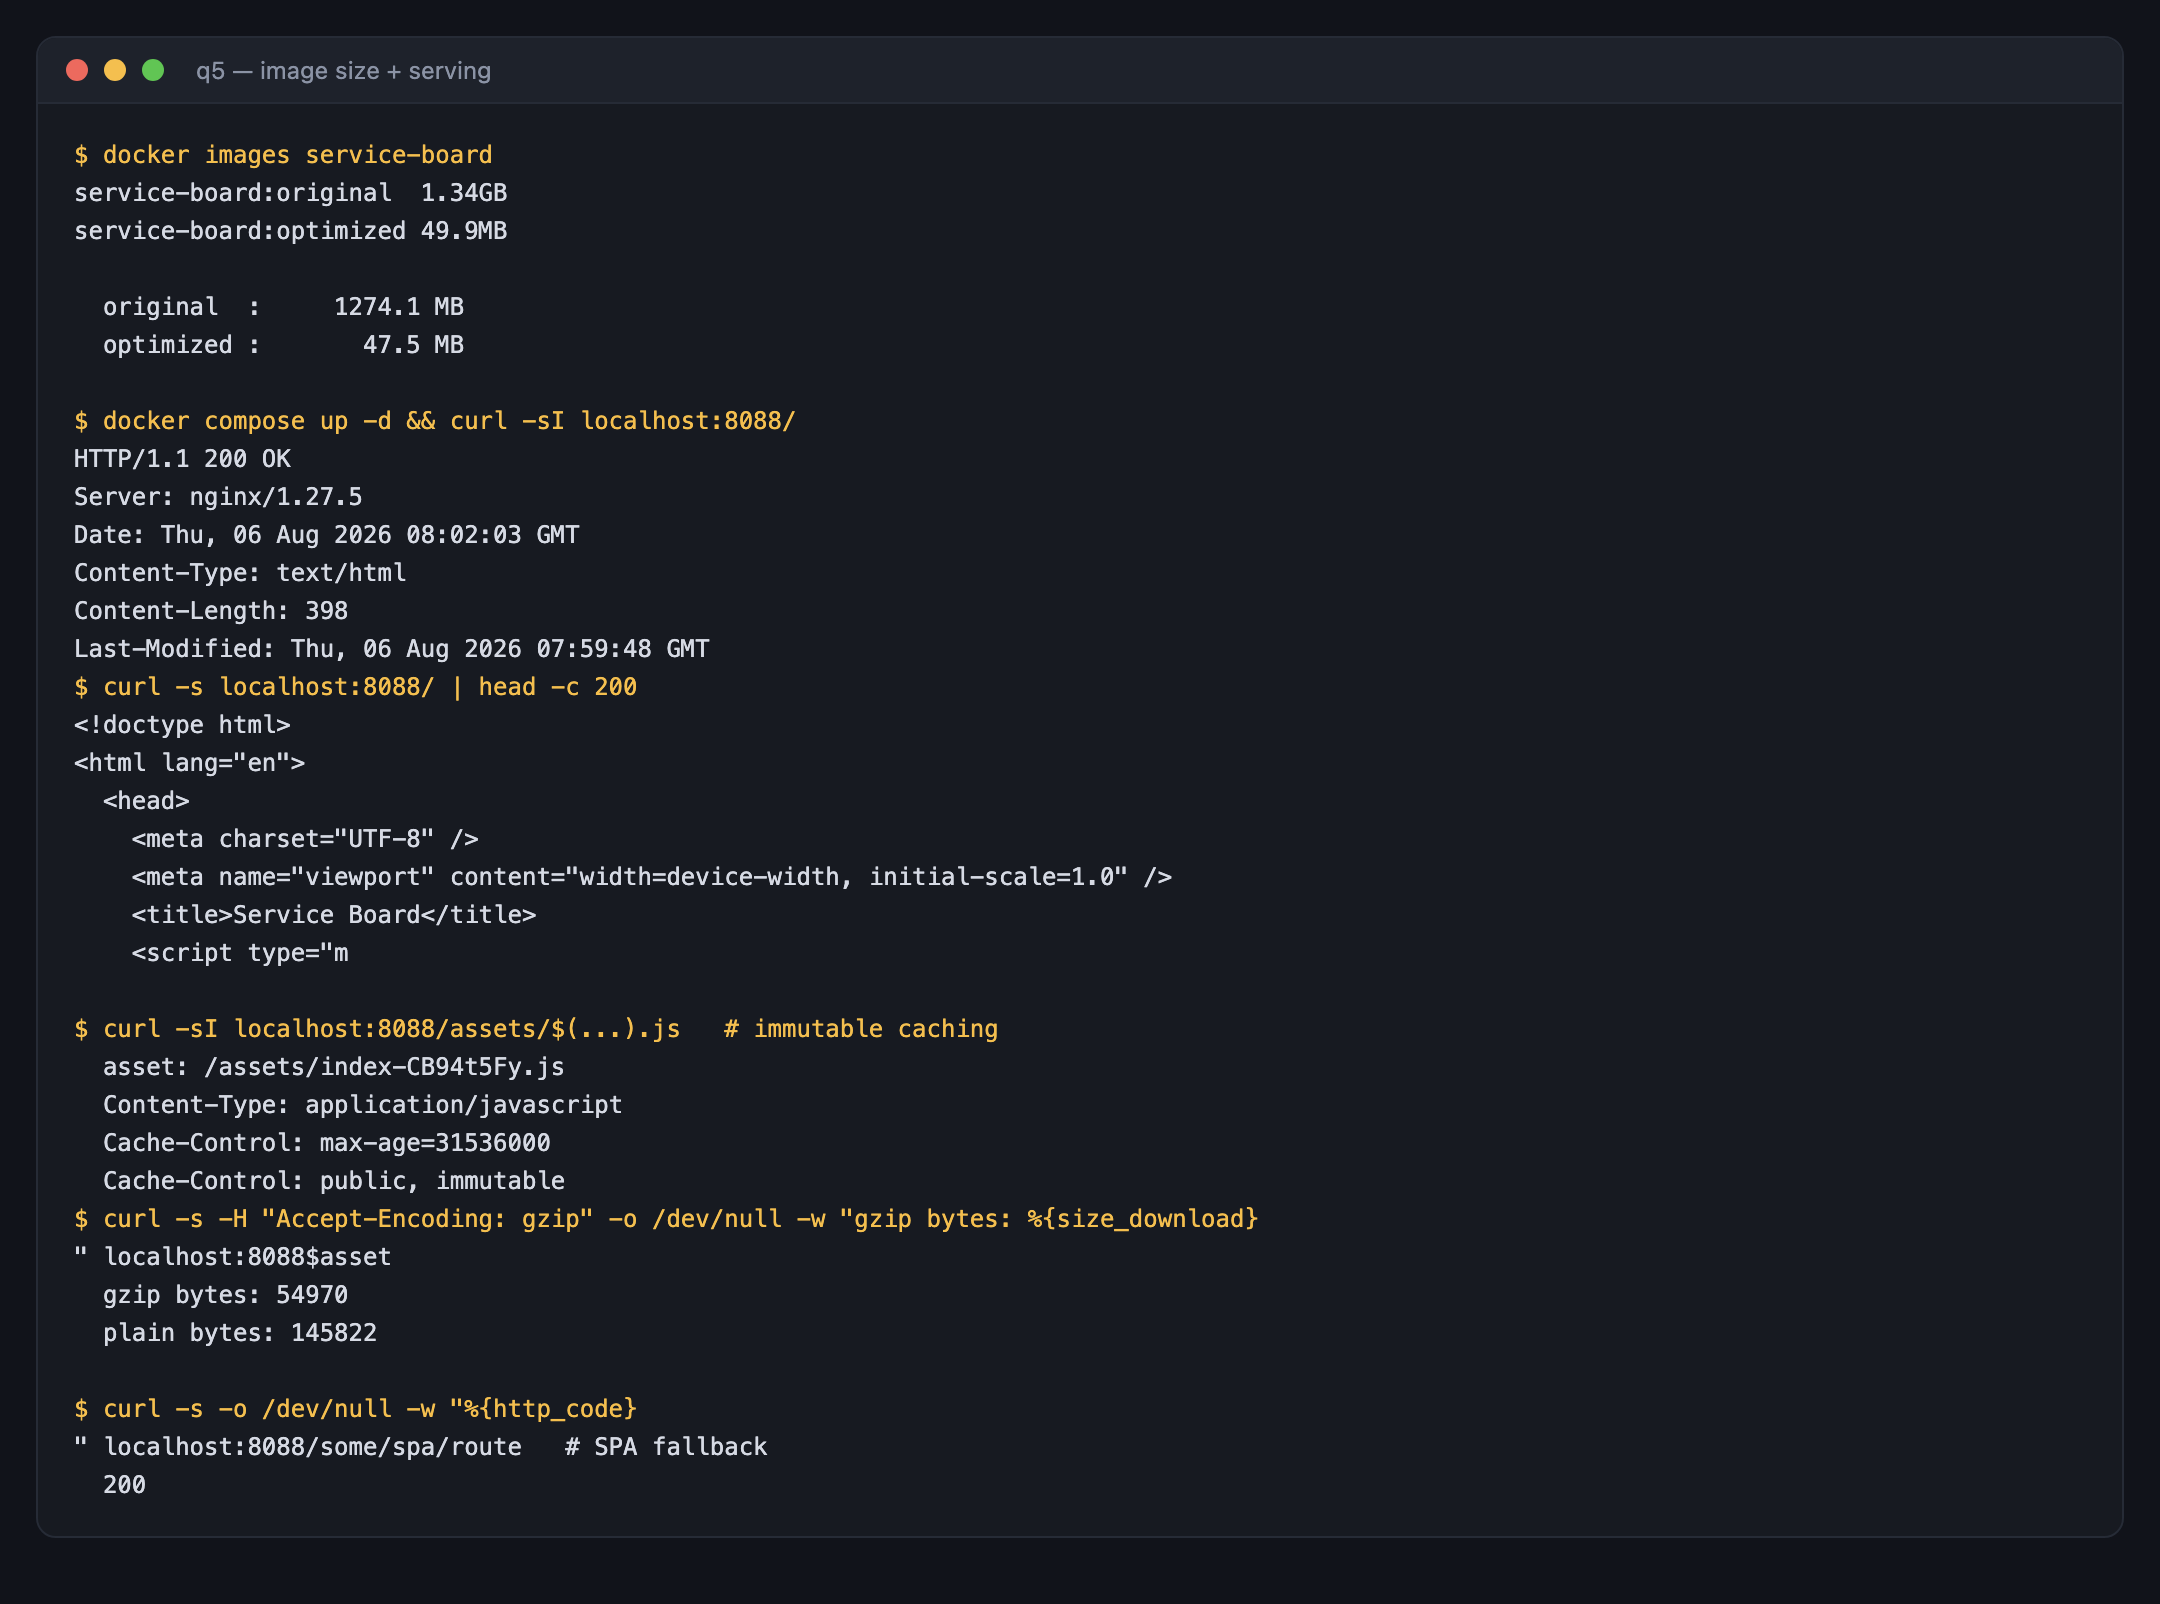
\includegraphics[width=0.94\textwidth]{figs/q5-size.png}
\caption{حجم دو ایمیج و بررسی سرویس‌دهی ایمیج بهینه: \lr{gzip}، کش تغییرناپذیر برای فایل‌های هش‌دار و \lr{fallback} مخصوص \lr{SPA}.}
\end{figure}

\begin{figure}[H]
\centering
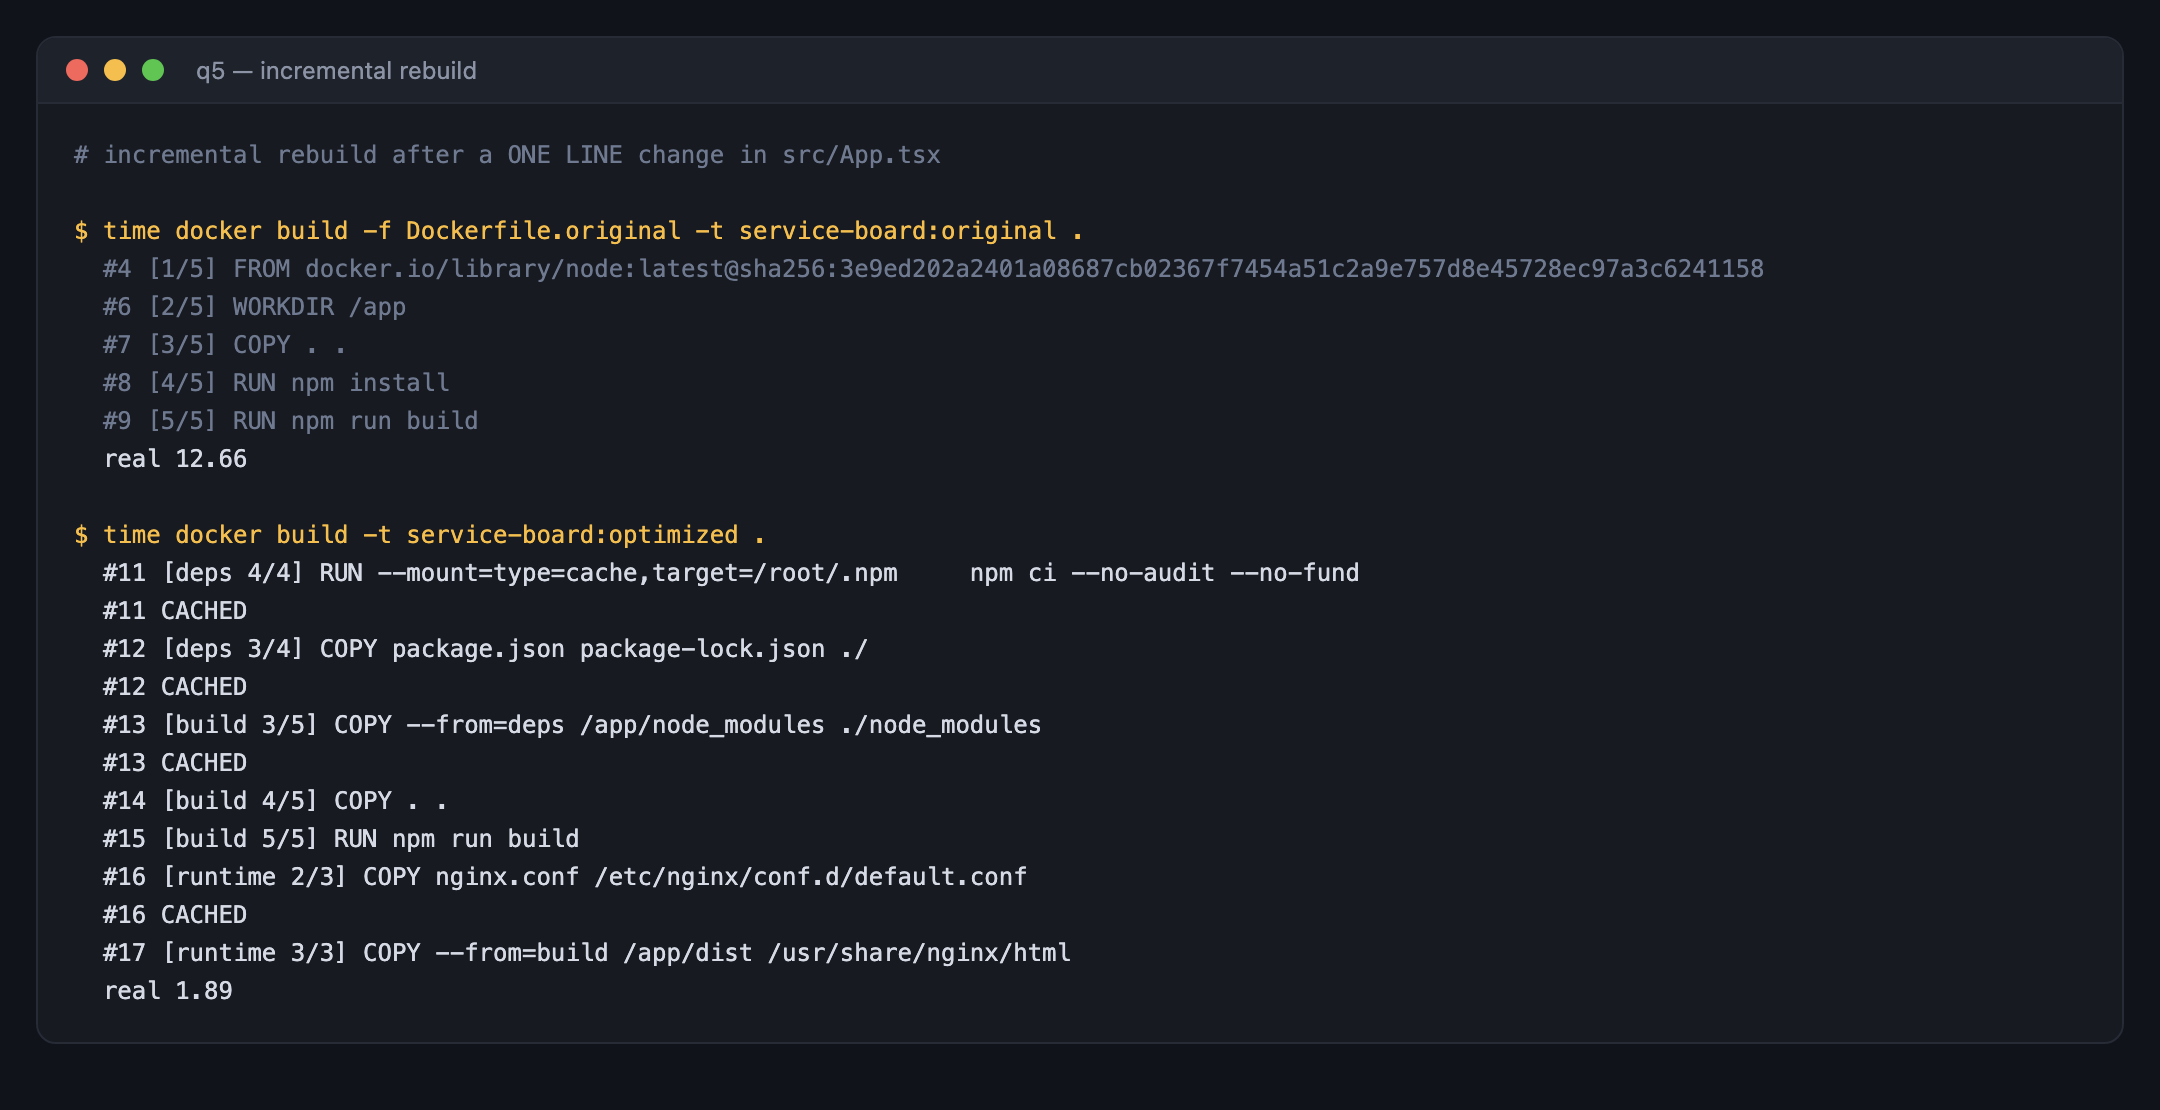
\includegraphics[width=0.94\textwidth]{figs/q5-rebuild.png}
\caption{بیلد مجدد پس از تغییر یک خط در \lr{src/App.tsx}: در نسخه‌ی اولیه \lr{npm install} دوباره اجرا می‌شود، در نسخه‌ی بهینه لایه‌ی وابستگی‌ها \lr{CACHED} می‌ماند.}
\end{figure}

\subsubsection*{توضیح تغییراتی که باعث بهینه‌سازی شدند}

\begin{enumerate}
	\item {بیلد چندمرحله‌ای}: بزرگ‌ترین عامل کاهش حجم. \lr{Node}، \lr{npm} و \lr{node\_modules} فقط در مراحل \lr{deps} و \lr{build} می‌مانند و به ایمیج نهایی راه پیدا نمی‌کنند؛ آنچه منتقل می‌شود تنها \lr{dist/} است (حدود ۱۵۰ کیلوبایت).
	\item {تعویض پایه‌ی زمان اجرا}: \lr{nginx:1.27-alpine} به‌جای \lr{node:latest}؛ برای فایل ایستا به \lr{Node} نیازی نیست و \lr{nginx} هم سریع‌تر و هم امن‌تر سرو می‌کند.
	\item {تگ‌های پین‌شده}: نتیجه‌ی بیلد امروز و سه ماه بعد یکی است.
	\item {ترتیب لایه‌ها}: \lr{package.json} و \lr{package-lock.json} جدا و {قبل} از سورس کپی می‌شوند؛ تا وقتی \lr{lockfile} عوض نشود، لایه‌ی نصب از کش می‌آید. این تنها دلیل کاهش \lr{12.7} ثانیه به \lr{1.9} ثانیه است.
	\item {\lr{npm ci} + \lr{cache mount}}: \lr{npm ci} دقیقا از \lr{lockfile} نصب می‌کند و \lr{--mount=type=cache} کش \lr{npm} را بین بیلدها نگه می‌دارد بدون اینکه داخل لایه‌ای ذخیره شود.
	\item {\lr{.dockerignore}}: \lr{node\_modules}، \lr{dist} و \lr{.git} از \lr{context} حذف شدند؛ هم ارسال \lr{context} سبک شد و هم باینری‌های میزبان به ایمیج نشت نمی‌کنند.
	\item {پیکربندی سرو}: \lr{gzip}، هدر \lr{Cache-Control: immutable} برای مسیر \lr{/assets/} (چون \lr{Vite} نام فایل‌ها را هش‌دار می‌سازد)، \lr{no-cache} برای \lr{index.html} و \lr{try\_files ... /index.html} برای مسیریابی سمت کلاینت. اندازه‌ی باندل اصلی از \lr{145 KB} به \lr{55 KB} روی شبکه کاهش یافت.
	\item {سخت‌سازی}: \lr{HEALTHCHECK}، فایل‌سیستم فقط‌خواندنی و \lr{no-new-privileges} در کامپوز.
\end{enumerate}

\pagebreak

\subsubsection*{\lr{docker-compose.yml} و \lr{nginx.conf}}

\begin{lstlisting}[language=Yaml]
services:
  web:
    build:
      context: .
      dockerfile: Dockerfile
      target: runtime
    image: service-board:optimized
    container_name: service-board
    restart: unless-stopped
    ports:
      - "${WEB_PORT:-8088}:80"
    healthcheck:
      test: ["CMD", "wget", "--spider", "-q", "http://127.0.0.1/"]
      interval: 10s
      timeout: 3s
      retries: 5
    read_only: true
    tmpfs:
      - /var/cache/nginx
      - /var/run
    security_opt:
      - no-new-privileges:true
\end{lstlisting}

\begin{lstlisting}[language=Nginx]
server {
    listen       80;
    server_name  _;
    root         /usr/share/nginx/html;
    index        index.html;

    gzip on;  gzip_vary on;  gzip_min_length 1024;
    gzip_types text/css text/plain application/javascript application/json image/svg+xml;

    location /assets/ {
        expires    1y;
        add_header Cache-Control "public, immutable";
        try_files  $uri =404;
    }

    location = /index.html { add_header Cache-Control "no-cache"; }

    location / { try_files $uri $uri/ /index.html; }
}
\end{lstlisting}
